\documentclass{beamer}

\usepackage[T2A]{fontenc}
\usepackage[utf8x]{inputenc}
\usepackage[english,bulgarian]{babel}
\usepackage{multirow}
\usepackage{ragged2e}

\mode<presentation> {
	\usetheme{Berlin}
}

%\usebackgroundtemplate {
%	\includegraphics[width=370px, height=270px, trim=0 0 0 -80px]{background}
%}

\graphicspath{{../images/}}

\title{Приближени пресмятания - подходи, методи, алгоритми}
\subtitle{Статистическа обработка на данни с R}

\author{Пламен Петров и Тодор Балабанов}

\date{6.VI.2020}

\institute[ЦО и ИИКТ към БАН] {
	Център за обучение \\
	Институт по информационни и комуникационни технологии \\ 
	Българската академия на науките \\
	\medskip
	\textit{p.petrov@iit.bas.bg todorb@iinf.bas.bg}
}

\addtobeamertemplate{navigation symbols}{}{
	\usebeamerfont{footline}
	\usebeamercolor[fg]{footline}
	\hspace{1em}
	\insertframenumber/\inserttotalframenumber
}

\begin{document}

\begin{frame}
	\titlepage
\end{frame}

\begin{frame}
\begin{exampleblock}{Acknowledgments}
\justify These teaching materials are funded by Velbazhd Software LLC and it is partially supported by the Bulgarian Ministry of Education and Science (contract D01–205/23.11.2018) under the National Scientific Program ``Information and Communication Technologies for a Single Digital Market in Science, Education and Security (ICTinSES)'', approved by DCM \# 577/17.08.2018.
\end{exampleblock}
\end{frame}

\section*{Теми}
\begin{frame}[shrink]
	\frametitle{Съдържание}
	\tableofcontents
\end{frame}

\section{Монте-Карло методи}

\begin{frame}
\center \huge{Монте-Карло методи}
\end{frame}

\subsection{Концепция за Монте-Карло пресмятания}

\begin{frame}
\frametitle{Стъпки за изчисление}
\begin{itemize}
	\item Определяне на област от допустими стойности

	\item Генериране на извадка от случайни числа в предварително дефинираната област

	\item Извършване на точни пресмятания с така генерираните случайни числа

	\item Обобщаване на резултатите от извършените пресмятания
\end{itemize}
\end{frame}

\begin{frame}
\frametitle{Пресмятане на числото $\pi$ с Монте-Карло метод}
\begin{figure}[]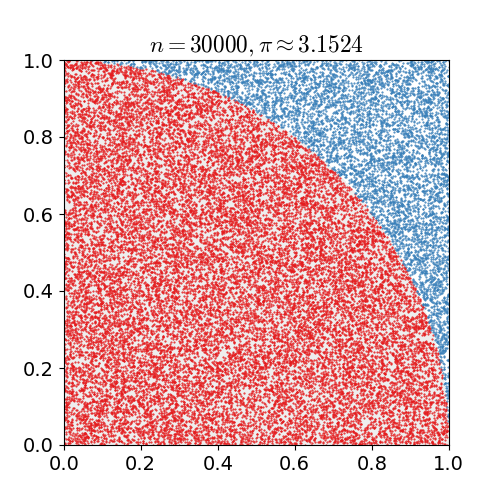
\includegraphics[width=\textwidth,height=0.75\textheight]{pic0060}\end{figure}
\end{frame}

\begin{frame}
\frametitle{Стъпки по примера}
\begin{itemize}
	\item Изчертаване на квадрат и четвъртина окръжност вписана в него

	\item Генериране на случайни равномерно разпределени числа, като координати (x,y двойки) в описаната допустима област

	\item Изброяване на точките с координати x,y които са на разстояние 1 от центъра на четвърт окръжността

	\item Съотношението между точките в четвърт окръжността и общия брой точки е $\pi/4$, което умножено по 4 дава приближена стойност за числото $\pi$ 
\end{itemize}
\end{frame}

\subsection{Прилагане на Монте-Карло в R}

\begin{frame}
\frametitle{Фактори силно влияещи на крайния резултат}
\begin{itemize}
	\item Ако генерираните случайни числа не са равномерно разпределени, това ще доведе до невярна апроксимация за търсената стойност

	\item Генерирането на малък брой координати за точки в дефиниционната област води до ниска надеждност на резултата от апроксимацията

	\item Колкото по-голям е броят на генерираните случайни числа, толкова по-надеждни са резултатите от апроксимацията
\end{itemize}
\end{frame}

\begin{frame}
\frametitle{Подготовка на извадката}
\begin{block}{Генериране на данни от хвърляне на зарове}
mode <- function(x) \{

	values <- unique(x)

	return( values[which.max(tabulate(match(x, values)))] )

\}

experiment <- function(n, d)\{

	x <- sample(6, n, TRUE)

	for(i in 2:d) \{
	
		x <- x + sample(6, n, TRUE)
		
	\}

	return( list($"$mean$"$=mean(x), $"$median$"$=median(x), $"$mode$"$=mode(x)) )

\}
\end{block}
\end{frame}

\begin{frame}
\frametitle{Извикване на функциите}
\begin{block}{Изпълнение на симулацията}
library( MonteCarlo )

result <- MonteCarlo(func=experiment, nrep=1000, param\_list=list($"$n$"$=c(10, 50, 100, 150, 200),$"$d$"$=c(1,2,6)))

summary( result );

MakeTable(output=result, rows=c($"$d$"$), cols=c($"$n$"$,$"$list$"$), digits=2, include\_meta=FALSE)
\end{block}
\end{frame}

\begin{frame}
\frametitle{Сравнение на средна, медиана и мода за експеримент със зарове}
\begin{table}[ht]
\centering\tiny
\begin{tabular}{ rrrrrrrrrrrrrrrrrrr }
\hline\hline\\\\
 list && \multicolumn{ 5 }{c}{ mean } &  & \multicolumn{ 5 }{c}{ median } &  & \multicolumn{ 5 }{c}{ mode } \\ 
d/n &  & 10 & 50 & 100 & 150 & 200 &  & 10 & 50 & 100 & 150 & 200 &  & 10 & 50 & 100 & 150 & 200 \\ 
 &  &  &  &  &  &  &  &  &  &  &  &  &  &  &  &  &  &  \\ 
1 &  & 10.50 & 10.48 & 10.49 & 10.50 & 10.50 &  & 10.52 & 10.50 & 10.48 & 10.50 & 10.52 &  & 10.48 & 10.50 & 10.42 & 10.49 & 10.53 \\ 
2 &  &  7.01 &  7.00 &  7.00 &  7.01 &  6.99 &  &  7.02 &  7.01 &  7.00 &  7.00 &  7.00 &  &  7.03 &  7.04 &  6.98 &  6.98 &  6.99 \\ 
6 &  & 20.94 & 21.03 & 21.00 & 21.01 & 21.00 &  & 20.90 & 21.01 & 20.99 & 21.00 & 21.00 &  & 20.86 & 20.98 & 21.04 & 21.00 & 20.97 \\ 
\\
\\
\hline\hline
\end{tabular}
\end{table}
\end{frame}

\section{Генетични алгоритми}

\begin{frame}
\center \huge{Генетични алгоритми}
\end{frame}

\subsection{Обща информация}

\begin{frame}
\frametitle{Същност}
\begin{itemize}
	\item Инструмент за евристична глобална оптимизация
	
	\item Популационно оранизирани
	
	\item Процес на еволюция

	\item Основно приложими при задачи с голяма размерност на пространството от решенията
\end{itemize}
\end{frame}

\begin{frame}
\frametitle{Основни операции}
\begin{itemize}
	\item Селекция на родители
	
	\item Кръстосване
	
	\item Мутация
	
	\item Оценка
\end{itemize}

Възможно е да се приложи правило за елита.
\end{frame}

\subsection{Практически пример}

\begin{frame}
\frametitle{Задача за раницата - данни}
\begin{table}[ht]
\centering
\begin{tabular}{|l|r|r|} 
  \hline
  Предмет & Ценност & Тегло \\ 
  \hline\hline
  cake & 10 & 1 \\
  \hline
  ice cream & 15 & 10 \\
  \hline
  orange juice & 10 & 5 \\
  \hline
  strawberries & 30 & 7 \\
  \hline
  grape & 30 & 1 \\
  \hline
  candies & 20 & 5 \\
  \hline
  chocolate & 2 & 1 \\
  \hline
\end{tabular}
\end{table}
\end{frame}

\begin{frame}
\frametitle{Структура от данни}
\begin{block}{Организация на информацията}
library( genalg )

data <- data.frame(item = c($"$cake$"$, $"$ice cream$"$, $"$orange juice$"$, $"$strawberries$"$, $"$grape$"$, $"$candies$"$, $"$chocolate$"$), points = c(10, 15, 10, 30, 30, 20, 2), weight = c(1, 10, 5, 7, 1, 5, 1))

limit <- 20

solution <- c(1, 0, 0, 1, 1, 0, 0)

data[solution==1, ]

cat(solution \%*\% data\$points)
\end{block}
\end{frame}

\begin{frame}
\frametitle{Оптималност на решенията}
\begin{block}{Целева функция}
fitness <- function(x) \{

	points <- x \%*\% data\$points

	weight <- x \%*\% data\$weight

	if (weight > limit) \{

		return( 0 )

	\} else \{

		return( -points )

	\}

\}
\end{block}
\end{frame}

\begin{frame}
\frametitle{Извършване на пресмятанията}
\begin{block}{Оптимизация на задачата за раницата с генетични алгоритми}
iterations <- 75

model <- rbga.bin(size=7, popSize=37, iters=iterations, mutationChance=0.01, elitism=TRUE, evalFunc=fitness)

cat( summary(model) )

best <- c(1, 0, 1, 1, 1, 1, 1)

data[best == 1, ]

cat(paste(best \%*\% data\$points, $"$/$"$, sum(data\$points)))
\end{block}
\end{frame}

\begin{frame}
\frametitle{Сходимост на процеса по оптимизация}
\begin{figure}[]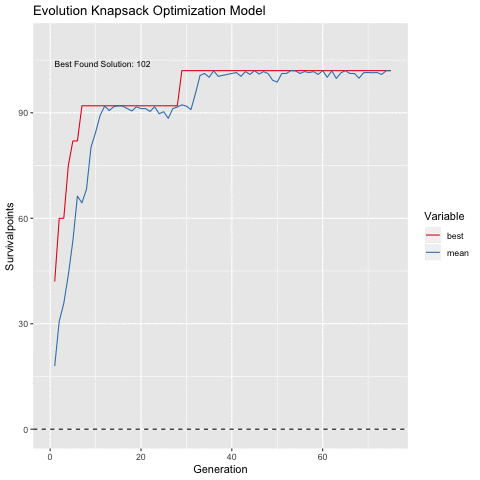
\includegraphics[width=\textwidth,height=0.75\textheight]{pic0061}\end{figure}
\end{frame}

\section{Изкуствени неверонни мрежи}

\begin{frame}
\center \huge{Изкуствени неверонни мрежи}
\end{frame}

\subsection{Обща информация}

\begin{frame}
\frametitle{Схема на биологична нервна клетка}
\begin{figure}[]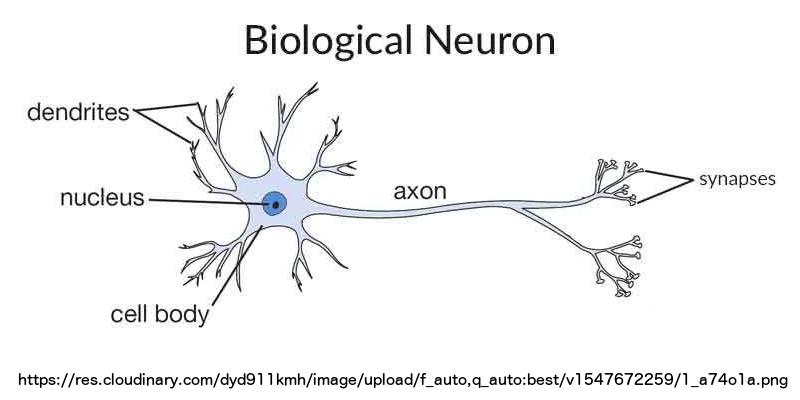
\includegraphics[width=\textwidth,height=0.75\textheight]{pic0062}\end{figure}
\end{frame}

\begin{frame}
\frametitle{Схема на изкуствен неврон}
\begin{figure}[]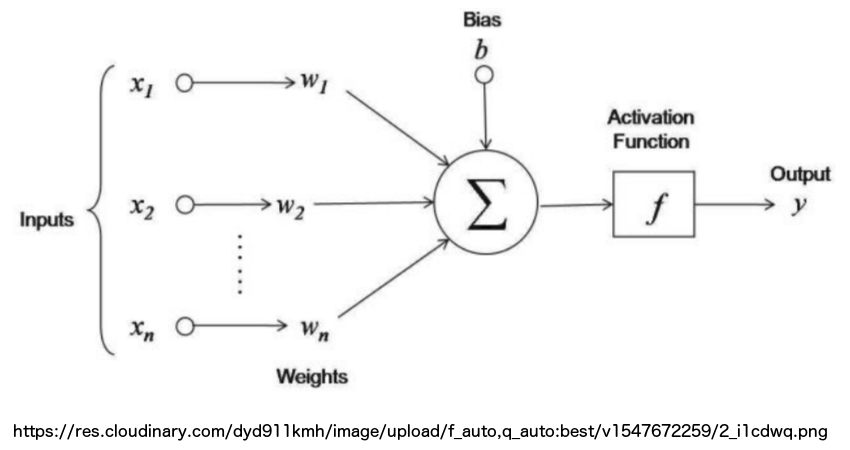
\includegraphics[width=\textwidth,height=0.75\textheight]{pic0063}\end{figure}
\end{frame}

\begin{frame}
\frametitle{Трансферна функция в изкуствен неврон}
\begin{equation}
y_i = \sum{(w_{ij}*y_j)} + b
\end{equation}
\end{frame}

\begin{frame}
\frametitle{Функции за активация на изкуствен неврон}
\begin{figure}[]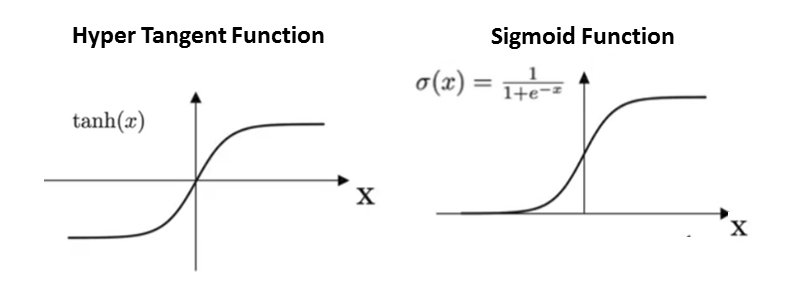
\includegraphics[width=\textwidth,height=0.75\textheight]{pic0064}\end{figure}
\end{frame}

\subsection{Практически пример}

\begin{frame}
\frametitle{Тренировъчно множество данни}
\begin{table}[ht]
\centering
\begin{tabular}{|l|r|r|} 
	\hline
	Technical Skills (TS) & Soft Skills (SS) & Successful Employment (SE) \\
	\hline\hline
	30 & 80 & Yes \\
	\hline
	10 & 20 & No \\
	\hline
	20 & 90 & Yes \\
	\hline
	30 & 40 & No \\
	\hline
	80 & 50 & Yes \\
	\hline
\end{tabular}
\end{table}
\end{frame}

\begin{frame}
\frametitle{Обучение с учител}
\begin{block}{Класифициране с изкуствена невронна мрежа}
library( neuralnet )

training <- data.frame(TS=c(30,10,20,30,80), SS=c(80,20,90,40,50), SE=c(1,0,1,0,1))

network <- neuralnet(SE~TS+SS, data=training, hidden=4, act.fct=$"$tanh$"$, linear.output=FALSE)

plot( network )

testing <- data.frame(TS=c(85,30,20), SS=c(10,20,75))

prediction <- compute(network, testing)

prediction\$net.result

ifelse(prediction\$net.result>0.5, TRUE, FALSE)
\end{block}
\end{frame}

\begin{frame}
\frametitle{Трислойна изкуствена невронна мрежа}
\begin{figure}[]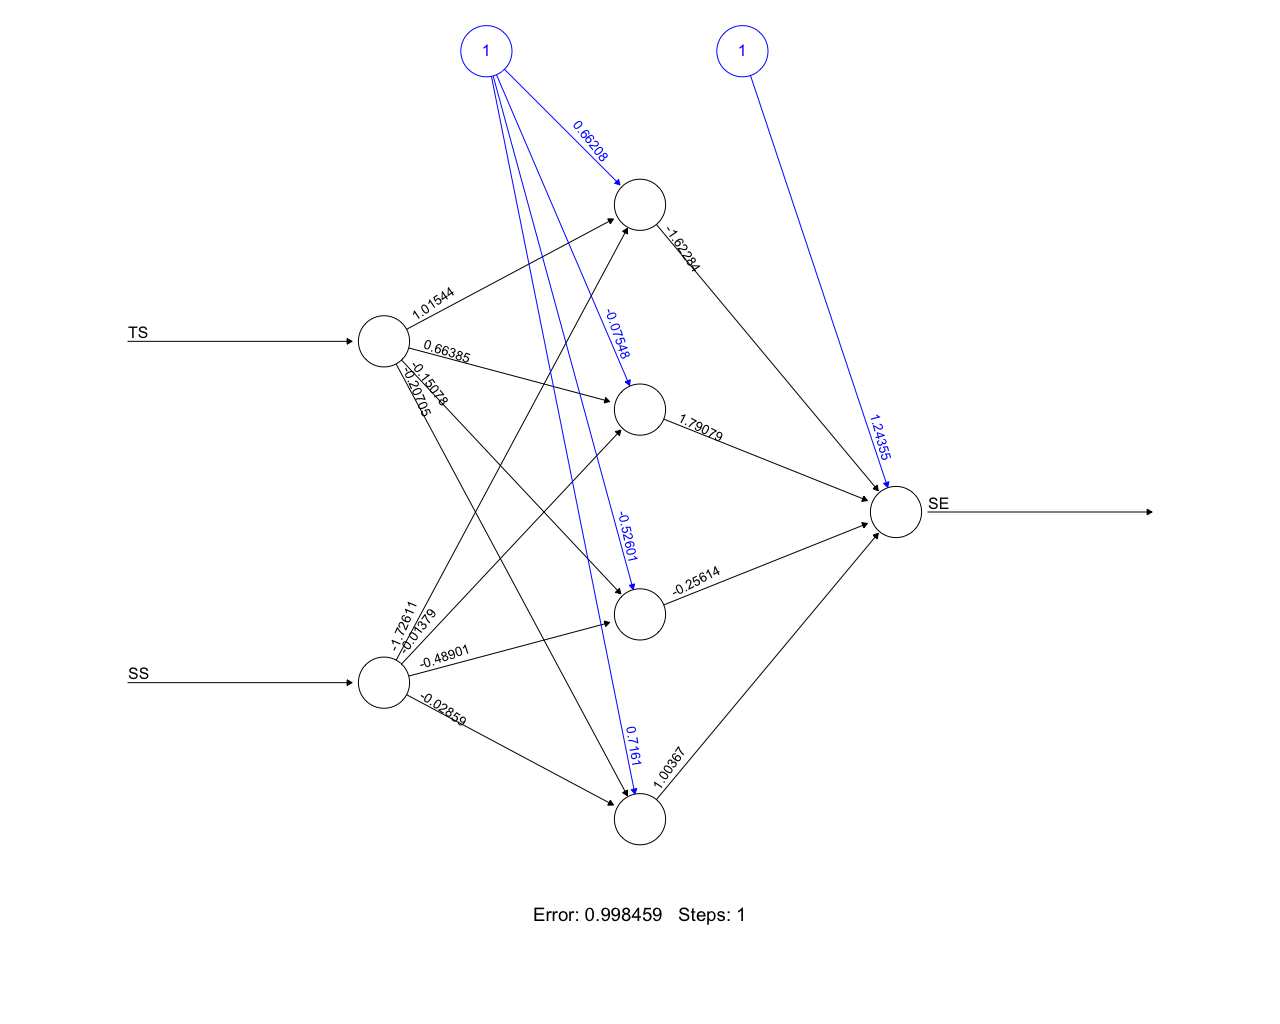
\includegraphics[width=\textwidth,height=0.75\textheight]{pic0065}\end{figure}
\end{frame}

\begin{frame}
\frametitle{Тестово множество данни}
\begin{table}[ht]
\centering
\begin{tabular}{|l|r|r|} 
	\hline
	Technical Skills & Soft Skills & Employment Forecast \\
	\hline\hline
	85 & 10 & 0.3322677 \\
	\hline
	30 & 20 & 0.3322677 \\
	\hline
	20 & 75 & 0.9924267 \\
	\hline
\end{tabular}
\end{table}
\end{frame}

\section{Заключение}

\begin{frame}
\center \huge{Заключение}
\end{frame}

\subsection{Дискусия}

\begin{frame}
\frametitle{Въпроси и отговори}
\center \huge{Благодаря за вниманието!}
\end{frame}

\end{document}
